% !TEX root=./main.tex

\documentclass[aspectratio=169]{beamer}

\usecolortheme{seahorse}

\usepackage{standalone}
\usepackage{amsmath} % for matrix example
\usepackage{upquote} % so single quotes can be directly pasted
\usepackage{xcolor}
\usepackage{pgfpages} % for seperating pages
\usepackage{algorithm,algorithmic}
\usepackage{minted}
\usepackage{multicol}
\usepackage{subfigure}
\usepackage{graphicx}
\usepackage[thinc]{esdiff}

\setbeameroption{show notes}
\setbeameroption{show notes on second screen=right}

\title{"Applying gradient filtering on joint optimization"}
\subtitle{Photo Realistic Rendering}
\author{Hyeonjang An}

\institute{
    GIST
}

\begin{document}
\setbeamertemplate{caption}{\raggedright\insertcaption\par}
\begin{frame}
\titlepage

\end{frame}

\begin{frame}{Outline}
    \tableofcontents
\end{frame}

\section{Intro}
    \subsection{Problem statement and Idea}
    \subsection{Related Work}
\section{Method}
    \subsection{Implementation of the previous work: Mesh case}
    \subsection{Laplacian operator on the image kernel}
    \subsection{The choice on step length}
\section{Result}
\section{Conclusion}

% 1. Problem statement
% !TEX root=../main.tex
\documentclass[beamer]{standalone}
\begin{document}

% introduction
\begin{frame}{Problem statement and Idea}
    \begin{itemize}
        \setlength\itemsep{1em}

        \item Problem 
        \begin{enumerate}
            \item ill-posed problem
            \item noisy gradient descent
            \begin{itemize}
                \item Monte-carlo differentiable rendering
                \item Stochastic gradient descent
            \end{itemize}
        \end{enumerate}
        \item Motivation
        \begin{enumerate}
            \item Observing gradient filtering behaviour on the joint optimization problem \\ 
            (texture and envmap)
        \end{enumerate}
        \begin{figure}
            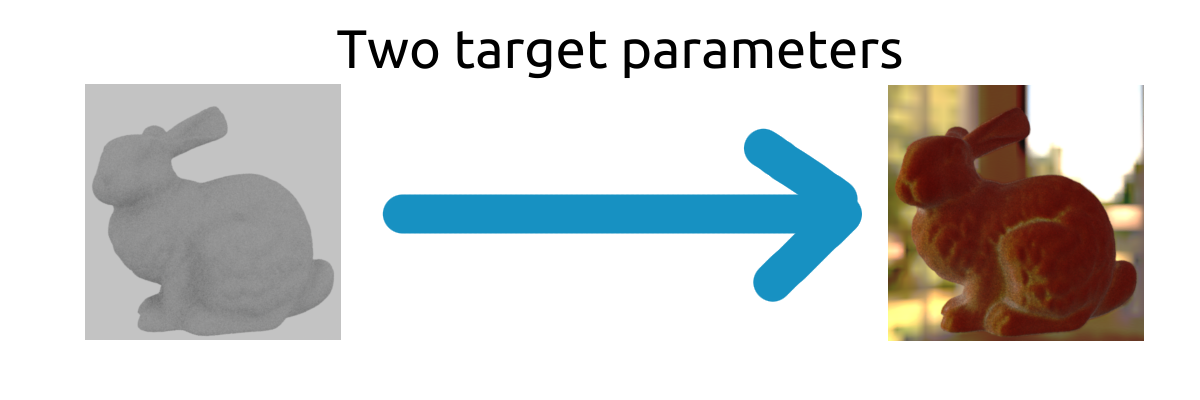
\includegraphics{./figures/Intro-1.png}
        \end{figure}
    \end{itemize}
\end{frame}
\end{document}

% 2. Related work explanation
% !TEX root=../main.tex
\documentclass[beamer]{standalone}
\begin{document}

% Differentiable rendering
\begin{frame}{Related-work}
\framesubtitle{Gradient Filtering}

\begin{itemize}
    \item "Laplacian Smooth Gradient Descent", Osher et al, 2019 ICLR
    \begin{figure}[h]
        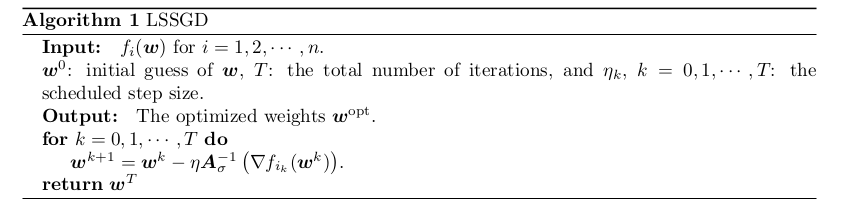
\includegraphics[width=0.8\linewidth]{./figures/related-work-1.png}
    \end{figure}
    \begin{enumerate}
        \item machine learning paper 
        \item smoothing method for stochastic gradient descent method (SGD) or GD
        \item multiplying the usual (stochastic) gradient by a one-dimensional discrete Laplacian
    \end{enumerate}

\end{itemize}

\note[item] {

    }
\end{frame}

% Mesh propertices / laplace
\begin{frame}{Related-work}
\framesubtitle{Gradient Filtering}
\begin{itemize}
    \item "Large steps in the Inverse Rendering", \\ 
    Baptiste Nicolet, Alec Jacobson and Wenzel Jackob, 2021 SIGGRAPH ASIA
    \begin{figure}[h]
        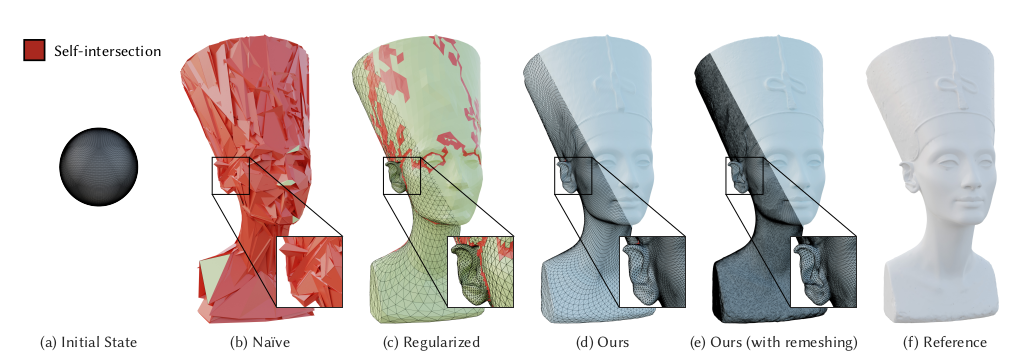
\includegraphics[width=0.8\linewidth]{./figures/related-work-2.png}
    \end{figure}
    \begin{enumerate}
        \item Quasi-Newton's method for gradient descent using the mesh properties
        \item Main idea: gradient filtering with the properties of paramters
    \end{enumerate}
\end{itemize}
    
% notes %
\note[item]{
    }   
\end{frame}
\end{document}


% 3-1.method part
% !TEX root=../main.tex
\documentclass[beamer]{standalone}
\begin{document}
% ==============================================================
% Method
% ==============================================================
\newminted{python}{fontsize=\scriptsize, 
		   linenos,
		   numbersep=8pt,
		   gobble=1,
		   frame=lines,
		   bgcolor=bg,
		   framesep=3mm} 

\defverbatim[colored]\exampleCode{
\begin{pythoncode}
   with torch.no_grad():
       # only the parameter vertex available
       l = igl.cotmatrix(v, f)
       m = igl.massmatrix(v, f, igl.MASSMATRIX_TYPE_BARYCENTRIC)
       # to pytorch
       l = torch.from_numpy(l.toarray()) 
       m = torch.from_numpy(m.toarray())

       # this is the same fomulation as laplacian smoothing
       i_L = (torch.eye(l.shape[1]) + 10*step_size * (m-10*l)).to(device='cuda')
       g = i_L.inverse() @ grad
   ...
   # reparameterization: x(u) = (I + \lambda L)_inv u
   param = l_p.inverse() @ param
\end{pythoncode}
}

\begin{frame}{Method}
\framesubtitle{Implementation of the previous work: Mesh case}
    \begin{itemize}
        \item iterative form
        \begin{equation}
                x \leftarrow x - \eta \textcolor{red}{(I + \lambda L)^{-p}} {\diffp{\Phi}{x}}
        \end{equation}
        \item Code
        \begin{itemize}
            \item Solve laplacian smoothing every iteration
        \end{itemize}
    \end{itemize}

    \exampleCode

% note %
\note[item]{
}
\end{frame}

\begin{frame}{Method}
    \framesubtitle{Implementation of the previous work: Mesh case}

        \begin{figure}
            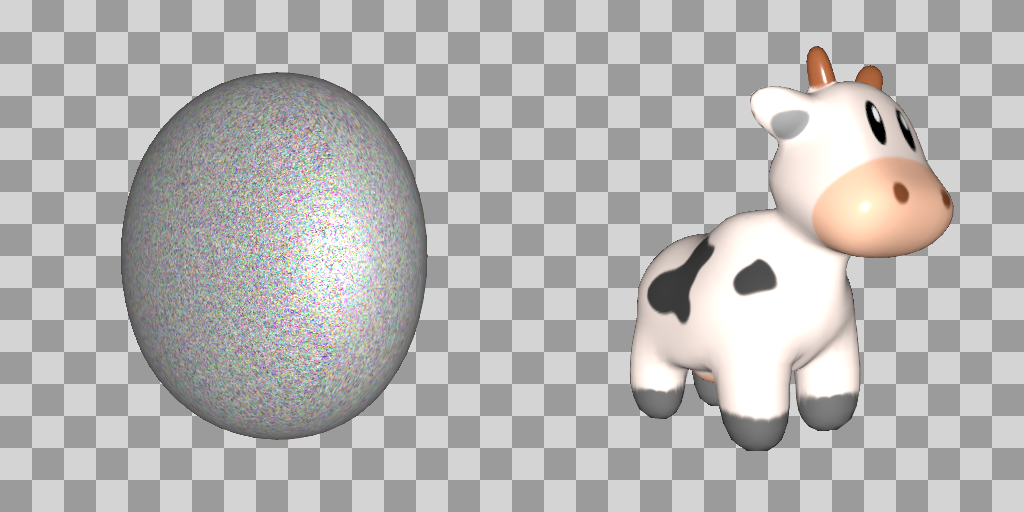
\includegraphics[width=0.25\linewidth]{./figures/spot.png}
        \end{figure}

        \begin{figure}
            \centering
            \begin{columns}[t]
                \column[]{.25\textwidth}
                    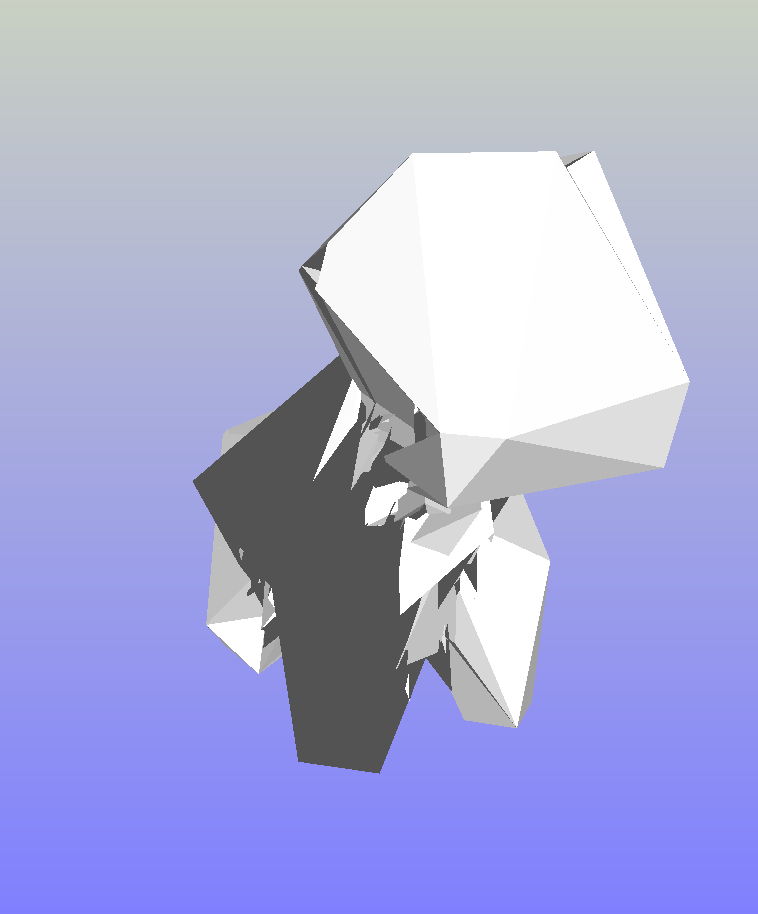
\includegraphics[width=\linewidth]{./figures/spot-raw.png}
                    \caption{Naive, 1000}

                \column[]{.25\textwidth}
                    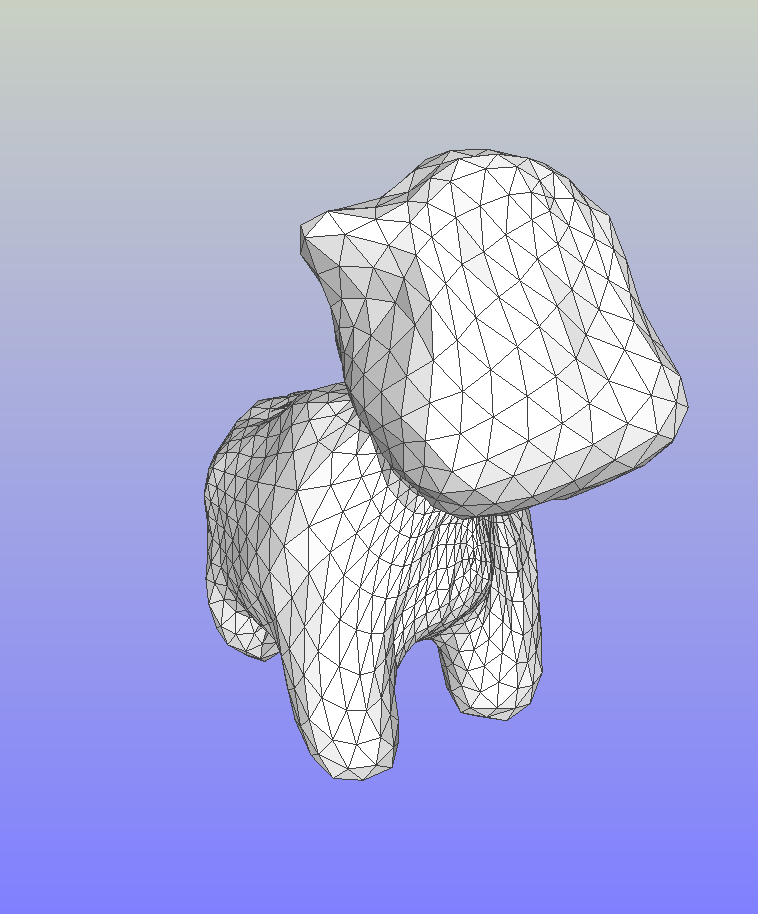
\includegraphics[width=\linewidth]{./figures/spot-reg.png}
                    \caption{Regularaization, 1000}

                \column[]{.25\textwidth}
                    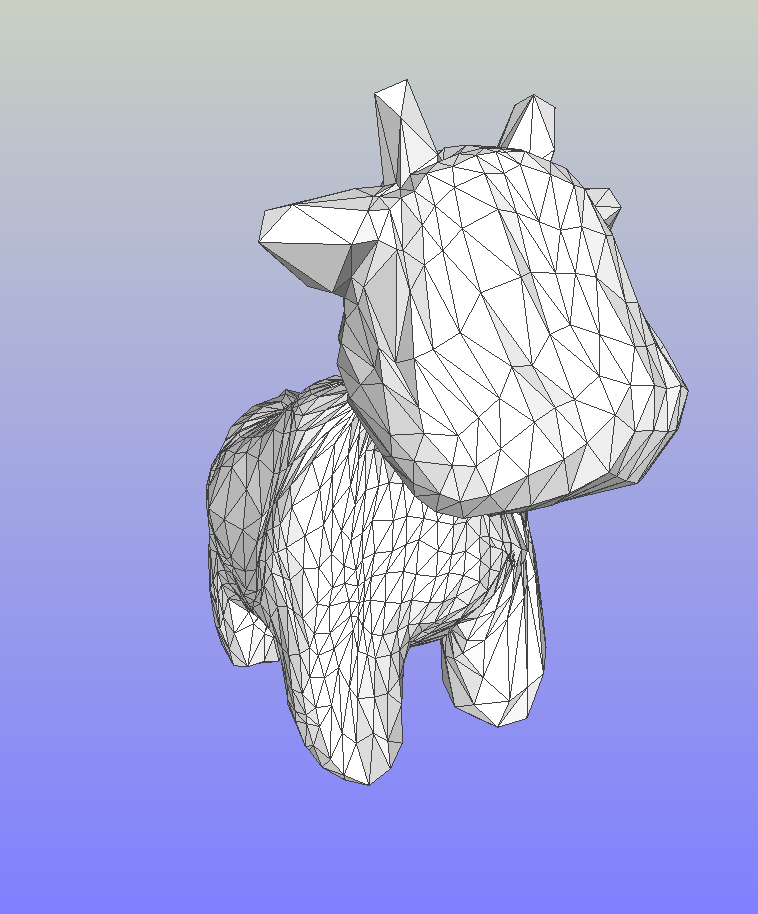
\includegraphics[width=\linewidth]{./figures/spot-new.png}
                    \caption{Gradient filtering, 100}
            \end{columns}
        \end{figure}

\end{frame}

\end{document}

% 3-2 method part
% !TEX root=../main.tex
\documentclass[beamer]{standalone}
\begin{document}
% ==============================================================
% Method : Gradient Descenet Explanations - 0 
% ==============================================================   
\begin{frame}{Method - Modified Gradient Descent}
    \framesubtitle{Conventional Gradient Descent}
        \begin{figure}[t]
            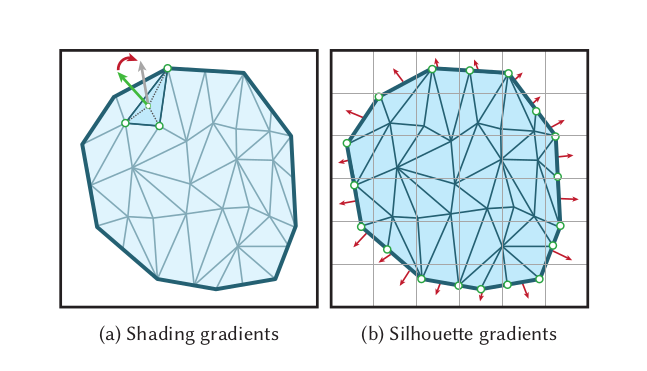
\includegraphics[width=8cm]{./figures/method1-figure-1.png}
        \centering
        \end{figure}
        \begin{itemize}    
            \item For Shading, small gradient steps are enough
            \item For Silhouette matching, large gradient steps are required!, but we will lose small gradient steps for shading
        \end{itemize}
    
    % note %
    \note[item] {
        First, I will explain the reason, why we cannot take easily large step length.

        As this picture, in differentiable rendering, small gradient steps are fine for shading.
        But, when the initial condition is awful like sphere, just topology is same, small gradient is not enough.
        
        Like silhouette mismatching cases, we need large gradient steps needed.
    }
\end{frame}

% ==============================================================
% Method : Gradient Descenet Explanations - 1 (no regularaization)
% ==============================================================    
\begin{frame}{Method - Modified Gradient Descent}
\framesubtitle{Conventional Gradient Descent}
\begin{itemize}
\item In the case of default object function (no regularization)
\begin{equation}
    minimize_{x\in\mathbb{R}^{nX3}}  \; \Phi(R(x))
\end{equation}
\item $x$ updating function by iterative precedure
\begin{equation}
    x \leftarrow x - \lambda \frac{\delta \Phi}{\delta x}
\end{equation}

\pause
\begin{figure}[t]
    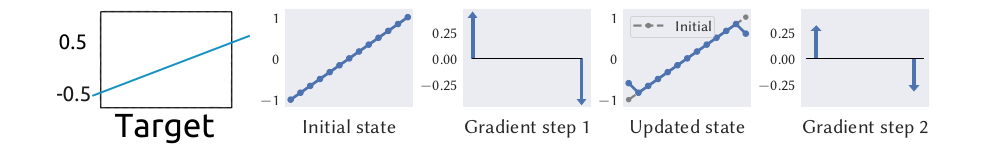
\includegraphics[width=0.8\textwidth]{./figures/method2-figure-1.png}
    \vspace*{-2mm}\caption{1D example of default}
\centering
\end{figure}

\end{itemize}

% note %
\note[item] {
    Our objective function is like this as we have already seen.
    So, iterative procedure for updating x will looks like this equation 4. Also, lambda is step length.

    Let's take this mesh example more simpler. like 1 dimensional case.
    Then, the result of toy example showed this plot
    Target is linear function between the interval -0.5 to 0.5

    As we can see, only silhouette takes far gradient, not smooth gradient.
    For solving this problem, until now the laplace regularaization is commonly used. 
}

\end{frame}
    
% ==============================================================
% Method : Gradient Descenet Explanations - 2 (only Laplacain regularization)
% ==============================================================    
\begin{frame}{Method - Modified Gradient Descent}
    \framesubtitle{Regularization}
    \begin{itemize}
    \item Adding laplace regularization
    \begin{equation}
        minimize_{x\in\mathbb{R}^{nX3}}  \; \Phi(R(x)) + \textcolor{red}{\frac{\lambda}{2} tr(x^{T}Lx)}
    \end{equation}
    
    \item $x$ updating function by iterative precedure
    \begin{equation}
        x \leftarrow x - \eta (\diffp{\Phi}{x}+\lambda L x)
    \end{equation}
    
    \begin{figure}[t]
        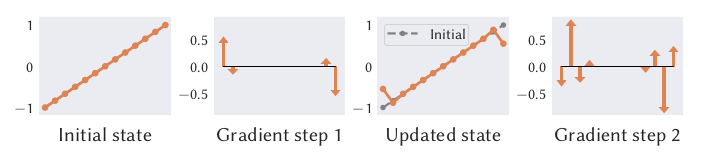
\includegraphics[width=0.65\textwidth]{./figures/method2-figure-2.png}
        \vspace*{-2mm}\caption{1D example of adding laplace}
        \centering
    \end{figure}
    \end{itemize}
    
    % note %
    \note[item] {
        This is the objective function added with laplace regularaizer.
        And this is the result of 1D example. It looks until not good.

        However, the important point of laplacian is that it has the property positive semi-definitive.
        If all the object term of x is positive definite, We can apply second-odrder optimization like newton method.
    }
    
\end{frame}
    
% ==============================================================
% Method : Gradient Descenet Explanations - 3 (Newton's Method)
% ==============================================================    
\begin{frame}{Method - Modified Gradient Descent}
\framesubtitle{Second-order Optimization}

\begin{itemize}
    \item Newton's method
    \begin{enumerate}
    \setlength\itemsep{0.5em}
        \item $tr(x^TLx)\ge0$ because L is positive-semidefinite by laplace properties
        \item objective terms are quadratic convex functions of x,
        \item a single step of Newton's method leads to the global optimum.
        \item Problem: expensive computation of Hessian
        \\ \emph{We need to calculate \alert{second-order derivate and its inverse term!}}
    \end{enumerate}

    \vspace*{1mm}
    \begin{equation}
        x \leftarrow 
        x - \eta (\diffp[2]{\Phi}{x}+\lambda L)^{-1} 
        (\diff{\Phi}{x}+\lambda L x)
    \end{equation}
    
    \pause

    \begin{figure}[t]
        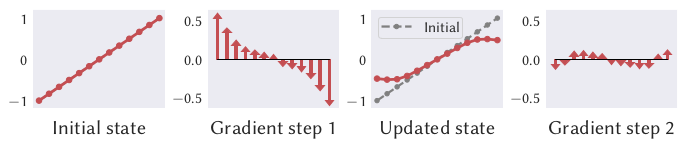
\includegraphics[width=0.65\textwidth]{./figures/method2-figure-3.png}
        \vspace*{-2mm}\caption{1D example of Newton's method}
    \centering
    \end{figure}
    \end{itemize}
    
    % note % 
    \note[item] {

        As before said, if all the object term of x is positive definite, We can apply second-order optimization like newton method.
        And by laplace property, the objective function is now positive definite

        It is well-known that Newton's method has a quadratic convergence speed. And it is much faster than other method.

        So, this is the result of newthod's method.
        The result of 1D example is much better.
        But, to solve this objective function, we need to calculate this hessian term and it's inverse.
        This is quite expensive computation if the problem has high dimensionality.
    }
\end{frame}

% ==============================================================
% Method : Gradient Descenet Explanations - 4 (Quasi-Newton explanation)
% ============================================================== 
\begin{frame}{Method - Modified Gradient Descent}
\framesubtitle{The explanation of Modified Gradient Descent}
\begin{itemize}
    \item Newton's method
    \begin{equation*}
        x \leftarrow 
        x - \eta ( 
            \textcolor{red}{ \diffp[2]{\Phi}{x} } + \textcolor{red}{\lambda L}
            )^{-1} (\diffp{\Phi}{x}+\lambda L x)
    \end{equation*}
    \item Quasi-Newton's method
    \begin{enumerate}
        \item Method to escape expensive computation of hessian and their inverse
        \item Use approximated hessian
        \item Identity matrix satisfies also hessain propertices for Newton's method (positive-definite, secant equation)
    \end{enumerate}
    \begin{equation}
        x \leftarrow
        x - \eta (
            \textcolor{red}{I} + \lambda L)^{-1} (\diffp{\Phi} {x} 
            + \textcolor{red}{\lambda L x}
            )
    \end{equation}
\end{itemize}
    
    % note %
    \note[item] {
        Therefore, the authors suggest the mesh version of Quasi-Newton's method.

        Quasi-Newton method is the modified newton method replacing the second-derivate, 
        which is Hessian, now approximated by Identity matrix.

        There are some well-known methods to replace hessian in numerical optimization.
        It is not represented in the paper.
        To approximate hessian, it is okay when the matrix satisfies positive-definite and secant equation conditions.
    }

\end{frame}

% ==============================================================
% Method : Gradient Descenet Explanations - 5 (Modified)
% ============================================================== 
\begin{frame}{Method - Modified Gradient Descent}
    \framesubtitle{Modified Gradient Descent}
    \begin{itemize}
        \item Modified Version
        \begin{enumerate}
            \item \emph{
                "Our goal is to benefit from accelerated convergence without compromising on minimizing $\Phi$, 
                hence we furthermore replace the last term in parantheses with the pure rendering gradient"
            }
            \item \emph{
                "In this way, we may view our descent as a form of sobolev or inverse-laplace preconditioning"
            }
            \item Modifying regularaization to sobolev preconditioned or inverse-laplace
        \end{enumerate}
        
        \begin{equation}
            x \leftarrow x 
            - \eta (I + \lambda L)^{-p} {\diffp{\Phi}{x}}
            %  \text{where p \ge 1, now p is 1, though p is possible to be 2}
        \end{equation}
    
        \begin{figure}[t]
            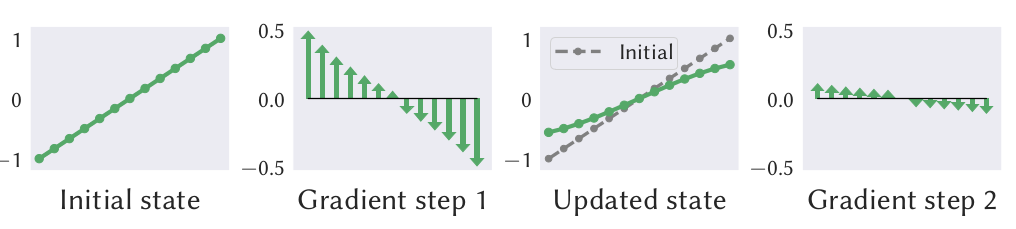
\includegraphics[width=0.65\textwidth]{./figures/method2-figure-4.png}
            \vspace*{-2mm}\caption{1D example of the modified version}
            \centering
        \end{figure}
    
    \end{itemize}
    
        % note %
        \note[item] {
            Moreover, the authors eliminate the previous regularization term following reason.
    
            It can be thought as they want not to remain any additional regularaizer.
            Also, they said that although omitting this last term, the behavior of regularization is retained, and also with large step sizes the convergence also be stabilized

            Through this modification, they takes the problem to a form of Sobolev or inverse-laplace preconditioning, which is the traditional method to optimize energy in geometry processing.
            
            I will pass this detail, i think it is hard for us. 
            just remember that they replace just adding regularization to using other gradient filtering method.

            And this is the result.
        }
    \end{frame}

% ==============================================================
% Method : Gradient Descenet Explanations - 6-1 (Diffusion reparameterization)
% ============================================================== 
\begin{frame}{Method - Modified Gradient Descent}
\framesubtitle{Diffusion reparameterization}

\begin{itemize}
\begingroup
\small
\item by head diffusion method...
\begin{equation}
    argmin_{x} \; \frac{1}{2} {||x-u||}^{2} + \lambda tr (x^{T}Lx)
\end{equation}

\item then by the solution of Euler-Lagrange equation\dots
\begin{equation}
    x = (I + \lambda L)^{-1} u
\end{equation}

\item then, the derivate to $u$
\begin{equation}
    \diffp{x}{u} = (I + \lambda L)^{-1}
\end{equation}

\item so, a single step $u$
\begin{equation}
    u \leftarrow u - \eta \diffp{x}{u} \diffp{\Phi}{x}
\end{equation}

\item together,
\begin{equation}
    x \leftarrow (I + \lambda L)^{-1} (u- \eta \diffp{x}{u} \diffp{\Phi}{x}) 
    = x - \eta(I + \lambda L)^{-2} \diffp{\Phi}{x}
\end{equation}
\endgroup

\item important, reparameterizing
\begin{equation}
    u = Lx
\end{equation}
\end{itemize}
% note %
\note[item]{
    Then this is the derive of inverse-laplace and Sobolev preconditioning form of their objective function by heat diffusion method.

    I will pass this details of explanation. 
    But the important point is here. We can derive this expression and this can be interpreted as reparameterizing the term x as u, the reparameterization, as before said.
}
\end{frame}

% ==============================================================
% Method : Gradient Descenet Explanations - 6-2 (Diffusion reparameterization)
% ============================================================== 
\begin{frame}{Method}
\framesubtitle{Diffusion reparameterization}
    Why this process (reparameterization) is necessary? \\
    - \alert{differential coordinate!}
    \begin{figure}
        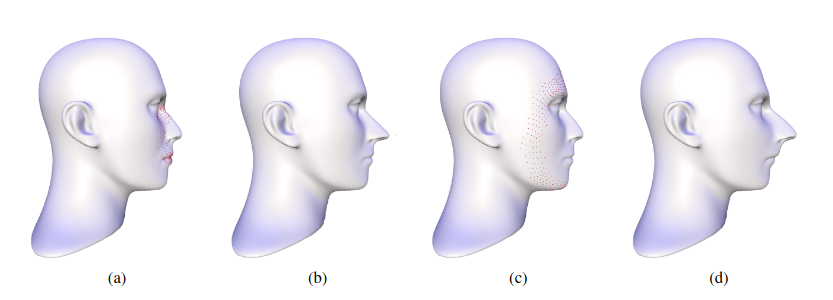
\includegraphics[width=\textwidth]{figures/differential_coordinate.png}
        \caption{Lipman, Yaron, et al. "Differential coordinates for interactive mesh editing." Proceedings Shape Modeling Applications, 2004.. IEEE, 2004.}
    \end{figure}
    
% note %
\note[item]{
   Why this process is needed? or important?

   Although this can be interpreted as many ways,

   to most easily understand, we can interpret this as differential coordinate.

   Roughly speaking, differential coordinate is not just moving vertex alone, move vertices with laplace propertices.
}
\end{frame}
\end{document}

% 3-3 method part
% !TEX root=../main.tex
\documentclass[beamer]{standalone}
\begin{document}
% ==============================================================
% Method : Gradient Descenet Explanations - 0 
% ==============================================================   
\begin{frame}{Method}
    \framesubtitle{Result: Gradient filtering on a texture - bug}
        \begin{figure}[t]
            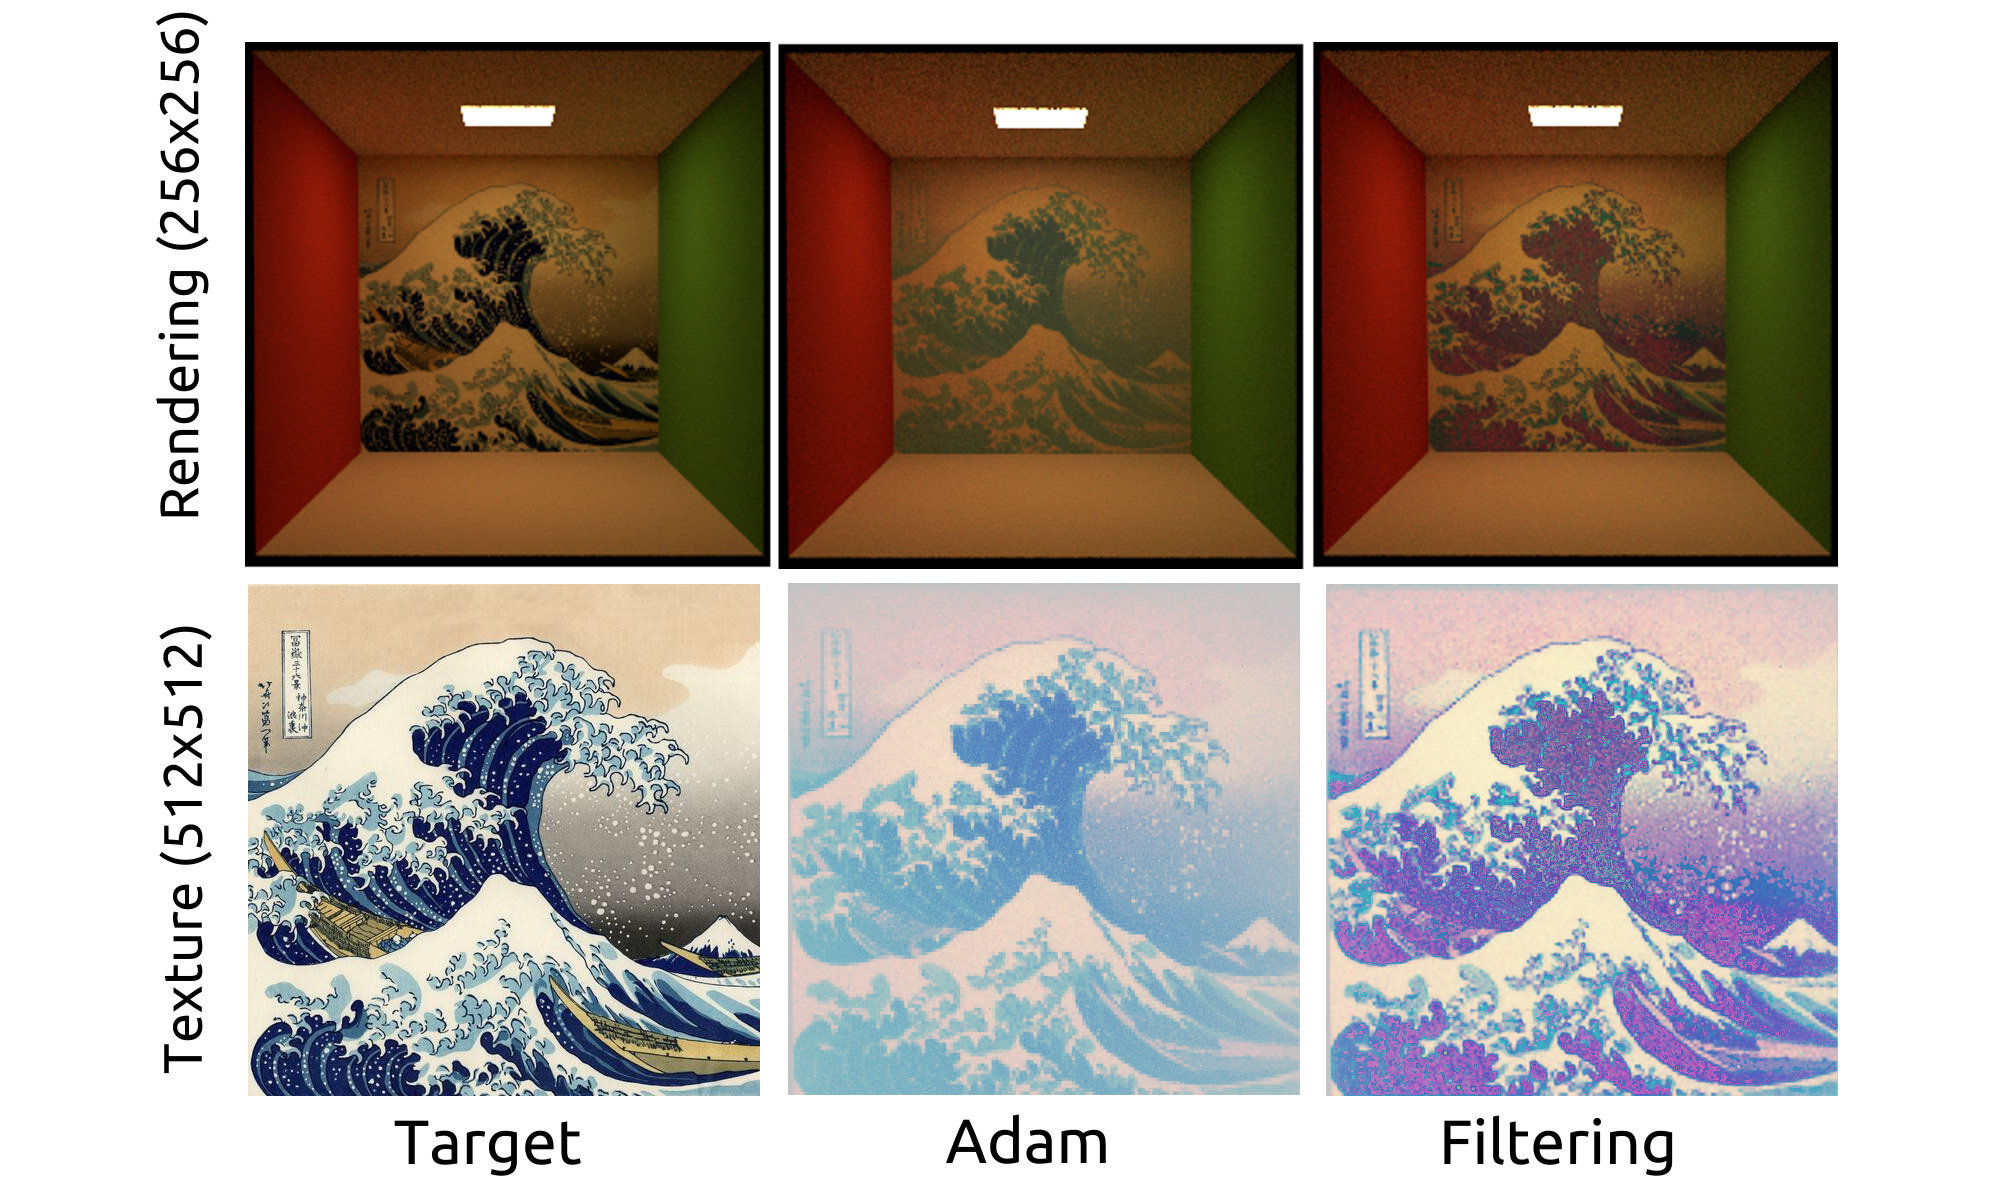
\includegraphics[width=6cm]{./figures/result-1.png}
        \centering
        \end{figure}
        \begin{itemize} 
            \item Currently, code has the bug
            \item MSE records
            \item learing rate: 0.5
        \end{itemize}
        \begin{table}
            \centering
            \resizebox{12cm}{!}{
            \begin{tabular}{ | c | c | c | c | c | c | c | c | c | c | c | c } \hline
                iter     & 1      & 2      & 3      & 4      & 5      & 6      & 7      & 8      & 9      & 10     \\\hline
                filter   & 0.1017 & \alert{0.0792} & 0.0625 & 0.0515 & 0.0462 & 0.0431 & 0.0412 & 0.0400 & 0.0393 & 0.0388 \\ \hline
                No       & 0.1016 & \alert{0.0912} & 0.0824 & 0.0752 & 0.0695 & 0.0650 & 0.0613 & 0.0584 & 0.0560 & 0.0540 \\ \hline  
            \end{tabular}}
        \end{table}
    % note %
    \note[item] {
    }
\end{frame}

% ==============================================================
% Method : Gradient Descenet Explanations - 1 
% ============================================================== 
\begin{frame}{Method}
    \framesubtitle{Result: Gradient filtering on a texture, Weigthed Gaussian Kernel version}
        \begin{figure}[t]
            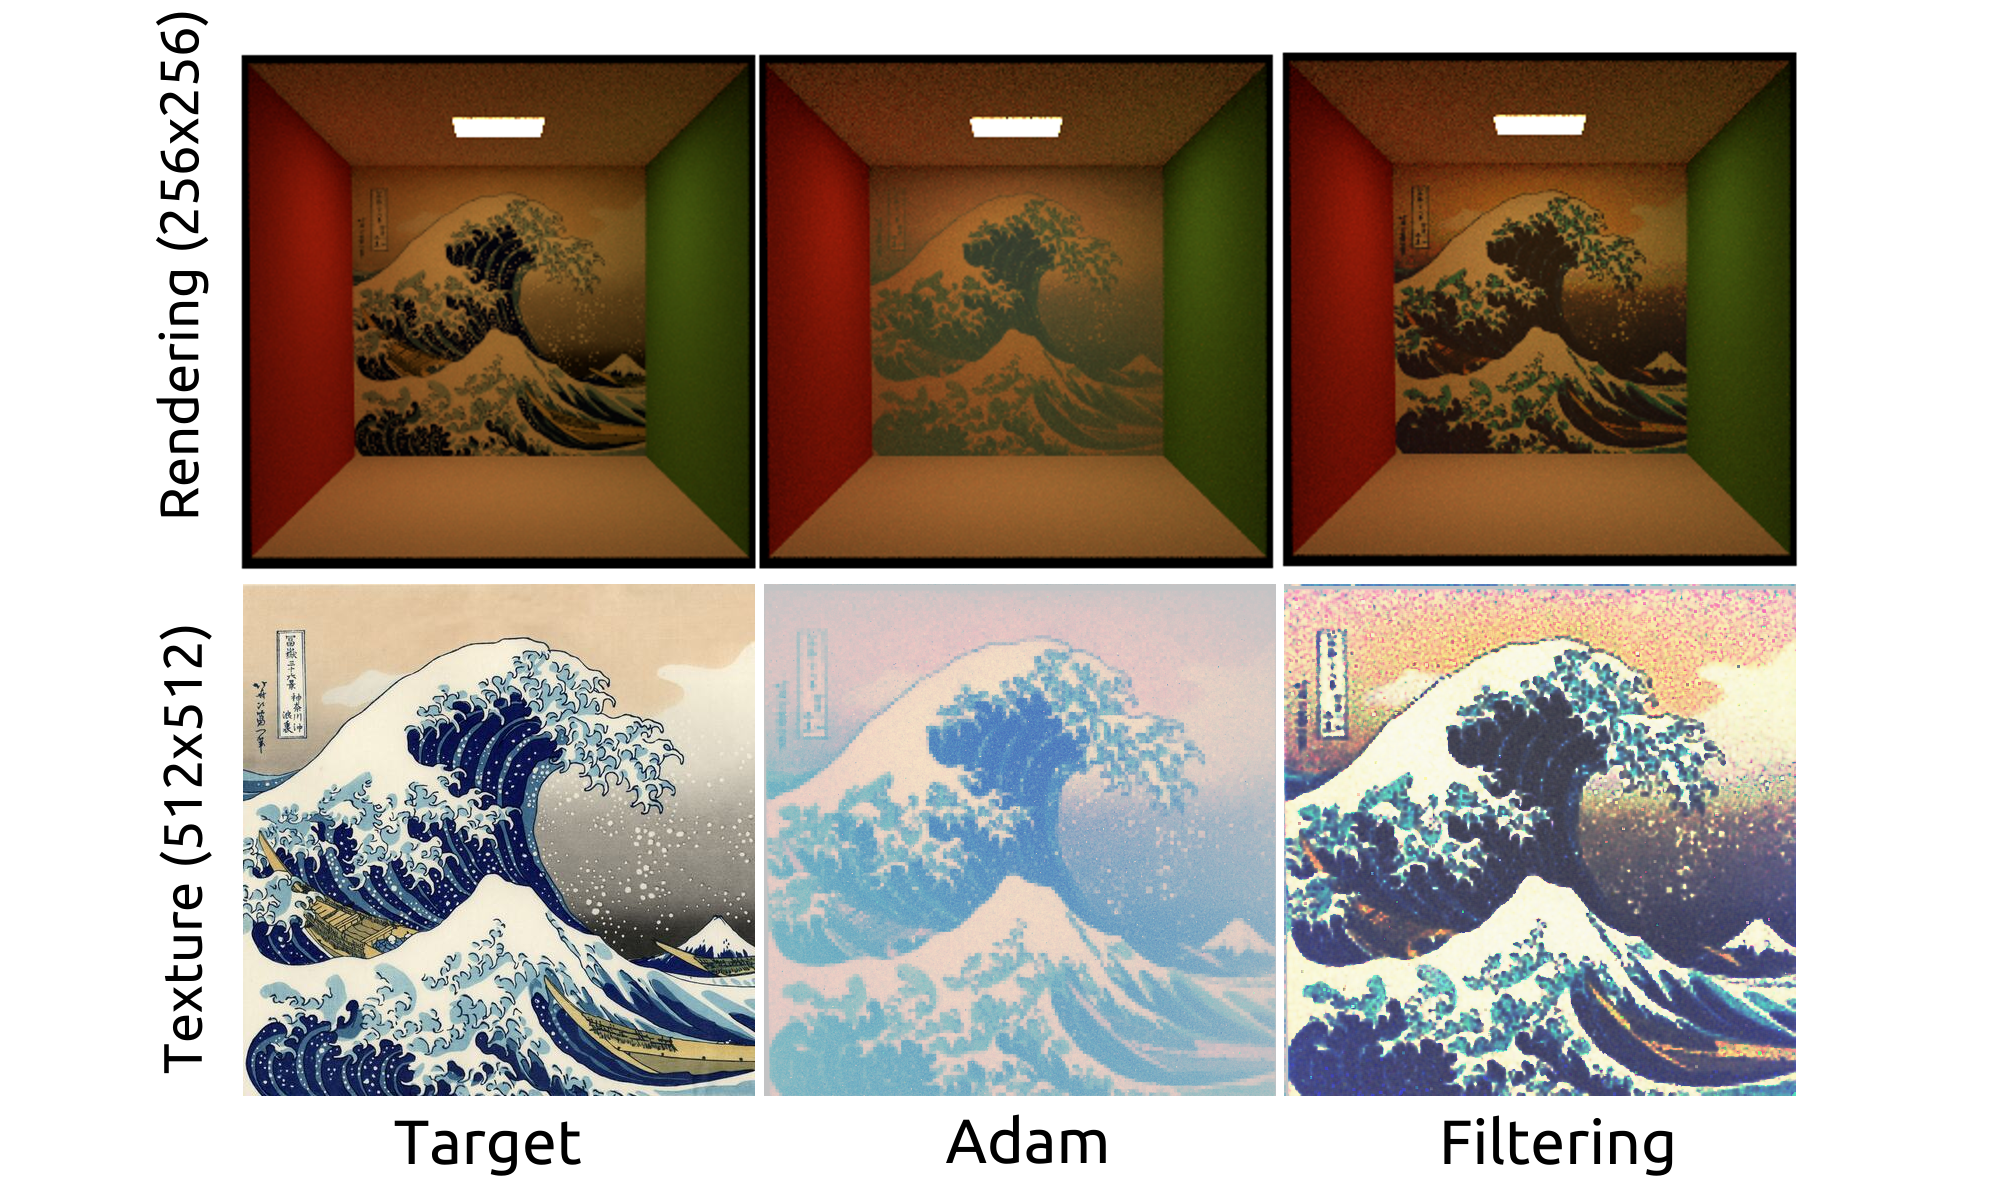
\includegraphics[width=6cm]{./figures/result-2.png}
        \centering
        \end{figure}
        \begin{equation}
            x \leftarrow x - \eta {(w*(D^{-1}G(x, \sigma)-D))}{\diffp{\Phi}{x}}
        \end{equation}
        \begin{itemize} 
            \item Whatever the laplacian operator is, if we want to filter the gradient, 
            the directly multiplying kernel reduce noise and weight give more step length
        \end{itemize}
        \begin{table}
            \centering
            \resizebox{12cm}{!}{
            \begin{tabular}{ | c | c | c | c | c | c | c | c | c | c | c | c } \hline
                filter   & 0.1017 & \alert{0.0593} & 0.0388 & 0.0301 & 0.0269 & 0.0262 & 0.0264 & 0.0269 & 0.0276 & 0.0282 \\ \hline
            \end{tabular}}
        \end{table}
    % note %
    \note[item] {
    }
\end{frame}

% ==============================================================
% Method : Gradient Descenet Explanations - 2
% ==============================================================   
\begin{frame}{Method}
    \framesubtitle{Result: Gradient filtering on a texture and environment map}
        \begin{figure}[t]
            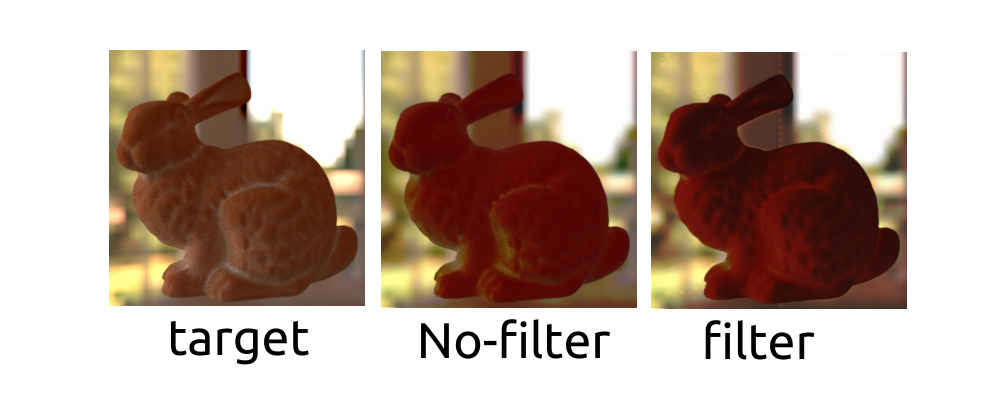
\includegraphics[width=\linewidth]{./figures/result-3.png}
        \centering
        \end{figure}
        \begin{itemize}    
            \item Bias problem, especially lighting by filtered environment map
            \item Bias is accumulated every iteration
        \end{itemize}
    
    % note %
    \note[item] {
    }
\end{frame}

% ==============================================================
% Method : Gradient Descenet Explanations - 3
% ==============================================================   
\begin{frame}{Method}
    \framesubtitle{Result: Gradient filtering on a environment map}
        \begin{figure}[t]
            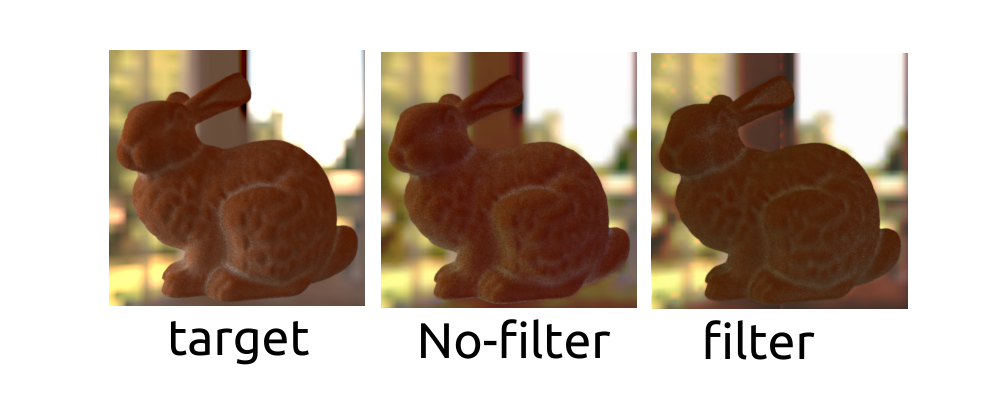
\includegraphics[width=\linewidth]{./figures/result-4.png}
        \centering
        \end{figure}
        \begin{itemize}
            \item Artifacts on lighting by filtered environment map
        \end{itemize}
    % note %
    \note[item] {
    }
\end{frame}

% ==============================================================
% Method : Gradient Descenet Explanations - 2
% ==============================================================   
\begin{frame}{Method}
    \framesubtitle{Result: Gradient filtering on a texture}
        \begin{figure}[t]
            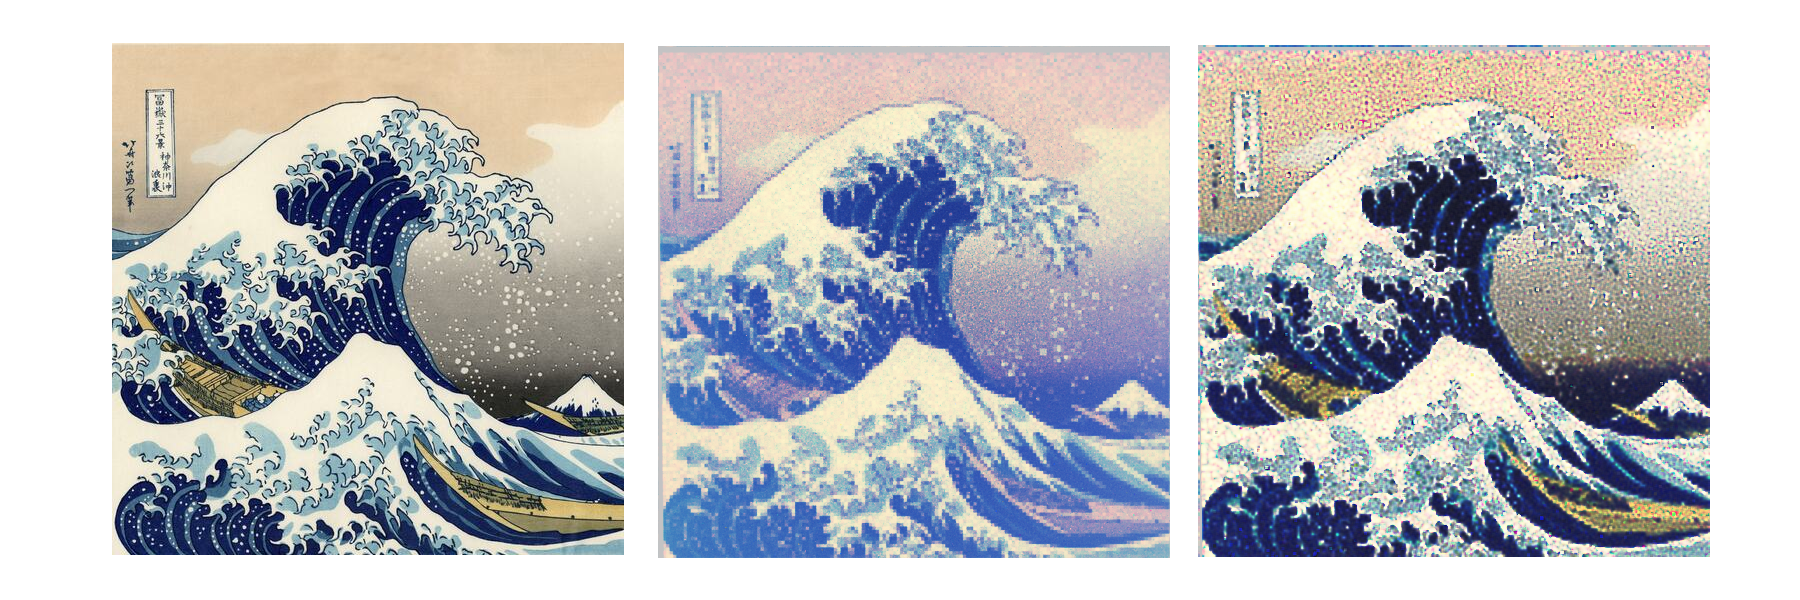
\includegraphics[width=\linewidth]{./figures/result-5.png}
        \centering
        \end{figure}
        \begin{itemize}    
            \item Bias is accumulated every iteration
        \end{itemize}
    
    % note %
    \note[item] {
    }
\end{frame}


\end{document}

% 4. conclusion
% !TEX root=../main.tex
\documentclass[beamer]{standalone}
\begin{document}
\begin{frame}{Summary}

\begin{itemize}
    \setlength\itemsep{1em}
    \item Gradient filtering using the known propertices on target parameters
    \item Test on the joint optimization problem, texture case
    \item Due to the bias (with the rougly designed gradient filtering), \\ 
    optimizing enviroment map shows a awful result
\end{itemize}
\end{frame}

\begin{frame}{Conclusion}

    \begin{itemize}
        \setlength\itemsep{1em}
        \item Gradient filtering makes the convergence faster
        \begin{itemize}
            \item reduce noise
            \item give a bigger step length
        \end{itemize}
        \item to global minimum, when properly applied 
        \item Not likely mesh, bias becomes bigger problem in the texture optimization procedure
    \end{itemize}
    
        % notes %
        \note[item]{
        }
        
    \end{frame}

    \begin{frame}{Q\&A}

        \note[item] {
            this is the end of the presentation
        }
    \end{frame}
\end{document}

\end{document}